%!TEX root = ../dissertation.tex

\hypertarget{(chap:capitolo6)}{}
\chapter{Tecnologie e strumenti}
Questo capitolo riporta le tecnologie e gli strumenti utilizzati durante il corso dello stage.
\section{Tecnologie}
\subsection{Python}
\begin{figure}[H]
	\begin{center} 
\includegraphics[width=2cm]{figures/python}
		\caption[Logo Python]{Logo Python} 
		\label{logo_python} 
	\end{center}
\end{figure}
\bit{Python}{python}, il cui logo riportato in Figura \ref{logo_python}, è un linguaggio di programmazione tra i più famosi attualmente disponibili, è un linguaggio ad oggetto, sintatticamente semplice e intuitivo che permette di avere un approccio ai problemi molto più operativo. \bit{Python}{python} è stata la base tecnologica su cui si è basato lo stage e gli strumenti utilizzati. Oltre ad aver usato questo linguaggio abbiamo utilizzato alcune librerie fornite dalla libreria standard.

\subsection{Google Or-Tools}
\begin{figure}[H]
	\begin{center} 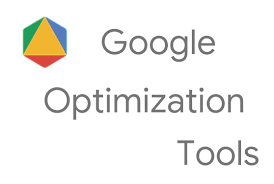
\includegraphics[width=4cm]{figures/google_or_tools}
		\caption[Logo Or-Tools]{Logo Or-Tools}  
		\label{logo_ortools} 

	\end{center}
\end{figure}
\bit{Google Or-Tools}{ortools}, il cui logo riportato in Figura \ref{logo_ortools}, è una libreria open source sviluppata da Google che permette di risolvere problemi di ottimizzazione potendo scegliere se utilizzare solver commerciali come \bit{CPLEX}{cplex} o \bit{Gurobi}{gurobi} oppure open source come \bit{SCIP}{scip} o \bit{Cbc}{cbc}. Inoltre viene fornita la libreria per diversi linguaggi come:
\begin{itemize}
	\item C++
	\item Java
	\item Python
	\item C\#
\end{itemize}
Nel nostro caso dato si è deciso di utilizzare la libreria per il linguaggio \bit{Python}{python}, utilizzandola per realizzare dei modelli di programmazione lineare intera. La libreria è stata imposta dall'azienda dopo il primo periodo di studio degli strumenti e delle tecnologie.

\subsection{Cbc}

\begin{figure}[H]
	\begin{center} 
\includegraphics[width=2cm]{figures/coin_banner}
		\caption[Logo Cbc]{Logo Cbc}  
		\label{logo_cbc} 
	\end{center}
\end{figure}
\bit{Cbc}{cbc}, il cui logo riportato in Figura \ref{logo_cbc}, è un solver di programmazione lineare intera scritto in \bit{C++}{cpp}, il motivo per cui si è scelto questo è la compatibilità con la libreria Google Or-Tools e la sua natura open source.

\subsection{Boost}
\begin{figure}[H]
	\begin{center} 
\includegraphics[width=5cm]{figures/boost}
		\caption[Logo Boost]{Logo Boost}
		\label{logo_boost} 
	\end{center}
\end{figure}
\bit{Boost}{boost}, il cui logo riportato in Figura \ref{logo_boost}, è un insieme di librerie \bit{C++}{cpp} open source che permettono di aumentare le capacità applicative del linguaggio. Viene utilizzato per progetti open source e commerciali. Il suo utilizzo si è reso necessario in quanto le librerie fornite dall'azienda dipendevano da esso, in particolare grazie alla capacità di esporre classi \bit{C++}{cpp} al linguaggio \bit{Python}{python}.

\subsection{Pandas}
\begin{figure}[H]
	\begin{center} 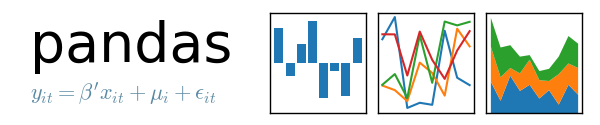
\includegraphics[width=5cm]{figures/pandas_logo}
		\caption[Logo Pandas]{Logo Pandas}
		\label{logo_pandas} 
	\end{center}
\end{figure}
\bit{Pandas}{pandas}, il cui logo riportato in Figura \ref{logo_pandas}, è una libreria open source utilizzata con il linguaggio \bit{Python}{python}, essa è fondamentale per eseguire analisi dei dati, inoltre offre delle funzionalità per la lettura dei dati da file xlsx,csv,txt e la manipolazione degli stessi. \\
Inoltre fornisce dei comodi metodi di scrittura su file anche verso \LaTeX, libreria consigliata dall'azienda.

\subsection{Matplotlib}
\begin{figure}[H]
	\begin{center} 
\includegraphics[width=5cm]{figures/matplotlib-1}
		\caption[Logo Matplotlib]{Logo Matplotlib}
		\label{logo_matplotlib} 
	\end{center}
\end{figure}
La libreria \bit{Matplotlib}{matplotlib}, il cui logo riportato in Figura \ref{logo_matplotlib}, è stata utilizzata durante lo stage per la realizzazione dei grafici e su di essa si basano le immagini 2D e 3D dei pacchi precedentemente mostrate, è stato fondamentale per poter eseguire una verificare quantitativa delle soluzioni. Inoltre è stata utilizzata per realizzare grafici importanti grazie ai quali spiegare in modo efficace alcuni concetti.

\subsection{Multiprocessing}
La libreria \bit{Multiprocessing}{multiprocessing} è stata utilizzata per seguire un numero maggiore di test in modo concorrente superando gli impedimenti del \glo{GIL}. Consigliata dall'azienda in quanto i tempi di esecuzione dei test non utilizzando la concorrenza si attestavano alle 10 ore circa, con la suddetta libreria ci attestiamo circa sulle 2 ore.

\section{Strumenti}
\subsection{Dropbox}
\begin{figure}[H]
	\begin{center} 
\includegraphics[width=5cm]{figures/dropbox_2017_logo}
		\caption[Logo Dropbox]{Logo Dropbox}  
		\label{logo_dropbox} 
	\end{center}
\end{figure}
\bit{Dropbox}{dropbox}, il cui logo riportato in Figura \ref{logo_dropbox}, è un servizio di archiviazione condivisa in cloud molto famoso e utilizzato nel mondo, permette di condividere file e documenti di vario genere con altri collaboratori, utile per la documentazione. Durante lo stage è stato utilizzato per condividere il diario e le presentazioni con i colleghi.

\subsection{GitHub}
\begin{figure}[H]
	\begin{center} 
\includegraphics[width=2cm]{figures/github-logo}
		\caption[Logo GitHub]{Logo GitHub}  
		\label{logo_github} 
	\end{center}
\end{figure}
\bit{GitHub}{github}, il cui logo riportato in Figura \ref{logo_github}, è un servizio di versionamento basato su repository \bit{git}{git}. Questo servizio permette di creare repository pubbliche e private con cui versionare il proprio progetto, aspetto improntante nello sviluppo software.

\subsection{Visual Studio Code}
\begin{figure}[H]
	\begin{center} 
\includegraphics[width=2cm]{figures/Visual_Studio_code}
		\caption[Logo Visual Studio Code]{Logo Visual Studio Code}
		\label{logo_vsc} 
	\end{center}
\end{figure}
\bit{Visual Studio Code}{visual}, il cui logo riportato in Figura \ref{logo_vsc}, è un editor open source che grazie alle estensioni installabili permette di utilizzare lo stesso editor per moltissimi linguaggi di programmazione. Inoltre grazie all'estensione per \bit{git}{git} è possibile versionare direttamente dall'editor, le estensioni permettono anche di eseguire una verifica della sintassi del codice su cui si lavora a livello statico in modo da individuare eventuali errori ed è integrato in esso il terminale con cui lanciare gli script \bit{Python}{python}.

\subsection{Jupyter Notebook}
\begin{figure}[H]
	\begin{center} 
\includegraphics[width=2cm]{figures/jupyter}
		\caption[Logo Jupyter Notebook]{Logo Jupyter Notebook}
		\label{logo_jupyter} 
	\end{center}
\end{figure}
\bit{Jupyter notebook}{jupyter}, il cui logo riportato in Figura \ref{logo_jupyter}, è applicazione web open source che permette di creare e condividere documenti che condividono del codice. Supporta molti linguaggi di programmazione tra i quali \bit{Python}{python} e permette una programmazione interattiva generalizzata dal tool \bit{IPython}{ipython}. Fondamentale per semplicità di utilizzo e per la possibilità di esportare gli script in molti formati.

\subsection{PIP}
\begin{figure}[H]
	\begin{center} 
\includegraphics[width=2cm]{figures/pip}
		\caption[Logo Pip]{Logo Pip}
		\label{logo_pip} 
	\end{center}
\end{figure}
\bit{PIP}{pip}, il cui logo riportato in Figura \ref{logo_pip}, è un gestore di pacchetti \bit{Python}{python} fondamentale per l'installazione di moduli non presenti nella libreria standard, di facile utilizzo ha permesso di installare velocemente moduli indispensabili per il proseguimento dello stage.

\subsection{Taiga}
\begin{figure}[H]
	\begin{center} 
\includegraphics[width=2cm]{figures/taiga}
		\caption[Logo Taiga]{Logo Taiga}
		\label{logo_taiga} 
	\end{center}
\end{figure}
\bit{Taiga}{taiga}, il cui logo riportato in Figura \ref{logo_taiga}, è una piattaforma di project management utilizzata durante il progetto per la gestione delle task da soddisfare in un certo periodo di tempo.